\documentclass[tikz,border=3.14mm]{standalone}
\usepackage{amsmath}
\usetikzlibrary{calc}

\begin{document}
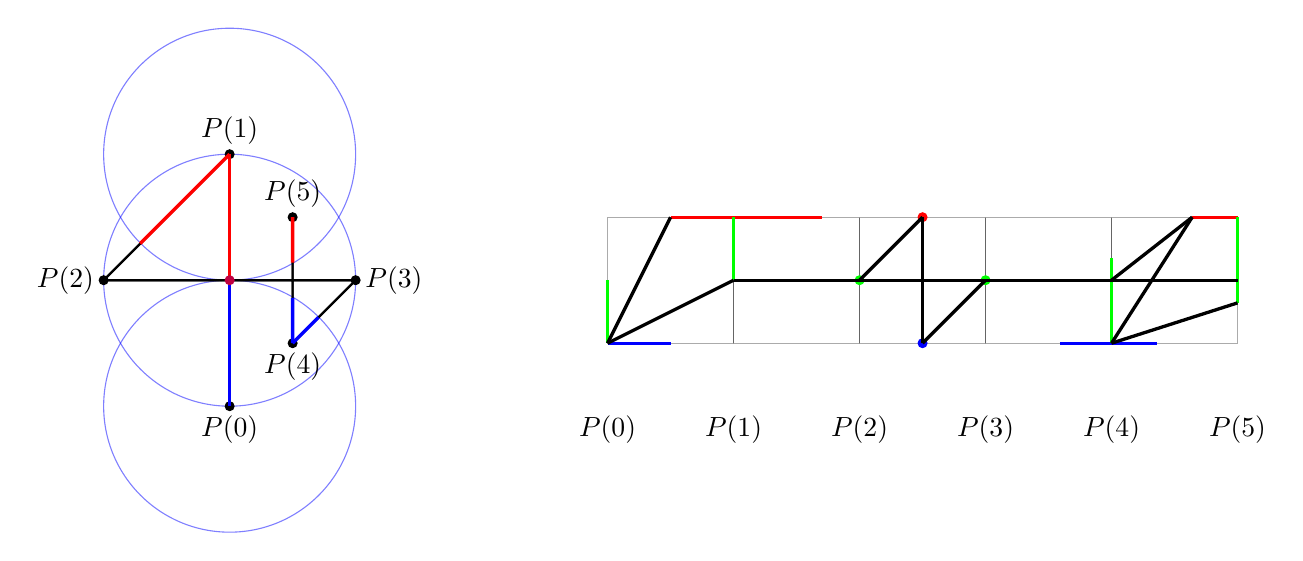
\begin{tikzpicture}[scale=0.8]

% Left side: Polyline with points and circle
\begin{scope}
    % Define points
    \coordinate (P0) at (0,0);
    \coordinate (P1) at (0,4);
    \coordinate (P2) at (-2,2);
    \coordinate (P3) at (2,2);
    \coordinate (P4) at (1,1);
    \coordinate (P5) at (1,3);
    
    % Draw blue circle
    \draw[blue, semitransparent] (P0) circle (2);
    \draw[blue, semitransparent] (P1) circle (2);
    \draw[blue, semitransparent] (0,2) circle (2);
    
    % Draw polyline
    \draw[black, thick] (P0) -- (P1) -- (P2) -- (P3) -- (P4) -- (P5);
    
    % Draw and label points
    \foreach \i in {0,...,5} {
        \filldraw (P\i) circle (2pt);
    }
		\node[below] at (P0) {$P(0)$};
		\node[above] at (P1) {$P(1)$};
		\node[left] at (P2) {$P(2)$};
		\node[right] at (P3) {$P(3)$};
		\node[below] at (P4) {$P(4)$};
		\node[above] at (P5) {$P(5)$};

    \draw[black, thick] (P0) -- (P1) -- (P2) -- (P3) -- (P4) -- (P5);

		\draw[blue, very thick] ($(P0)!0!(P1)$) -- ($(P0)!0.5!(P1)$);
		\draw[blue, very thick] ($(P3)!0.59!(P4)$) -- ($(P3)!1!(P4)$);
		\draw[blue, very thick] ($(P4)!0!(P5)$) -- ($(P4)!0.36!(P5)$);

		\draw[red, very thick] ($(P0)!0.5!(P1)$) -- ($(P0)!1!(P1)$);
		\draw[red, very thick] ($(P1)!0!(P2)$) -- ($(P1)!0.71!(P2)$);
		\draw[red, very thick] ($(P4)!0.64!(P5)$) -- ($(P4)!1!(P5)$);

		\filldraw[purple] (0,2) circle (2pt);
\end{scope}

% Right side: Rectangle with 5 squares
\begin{scope}[xshift=6cm, yshift=1cm]
    % Define square size
    \def\sqsize{2}
    
    % Draw 5 squares in a row with semi-transparent gray outlines
    \foreach \i in {0,...,4} {
        \draw[black!80, semitransparent] (\i*\sqsize,0) rectangle (\i*\sqsize+\sqsize,\sqsize);
				\node[below] at (\sqsize*\i, -1) {$P(\i)$};
    }
		\node[below] at (\sqsize*5, -1) {$P(5)$};
    
    % Optional: Draw the outer rectangle outline (can be removed if not needed)
    \draw[gray!50, semitransparent] (0,0) rectangle (5*\sqsize,\sqsize);


		\draw[blue, very thick] (0,0) -- (\sqsize*0.5,0);
		\draw[blue, very thick] (\sqsize*3.59,0) -- (\sqsize*4.36,0);
		\filldraw[blue] (\sqsize*2.5,0) circle (2pt);

		\draw[red, very thick] (0.5*\sqsize,\sqsize) -- (\sqsize*1.70,\sqsize);
		\draw[red, very thick] (\sqsize*4.64,\sqsize) -- (\sqsize*5,\sqsize);
		\filldraw[red] (\sqsize*2.5,\sqsize) circle (2pt);


		\draw[green, very thick] (\sqsize*0,0*\sqsize) -- (\sqsize*0,0.5*\sqsize);
		\draw[green, very thick] (\sqsize,0.5*\sqsize) -- (\sqsize,\sqsize);
		\filldraw[green] (\sqsize*2,\sqsize*0.5) circle (2pt);
		\filldraw[green] (\sqsize*3,\sqsize*0.5) circle (2pt);

		\draw[green, very thick] (\sqsize*4,0*\sqsize) -- (\sqsize*4,0.68*\sqsize);
		\draw[green, very thick] (\sqsize*5,0.32*\sqsize) -- (\sqsize*5,1*\sqsize);


		\draw[black, very thick] (0,0) -- (\sqsize*0.5,1*\sqsize);
		\draw[black, very thick] (0,0) -- (\sqsize*1,0.5*\sqsize);
		\draw[black, very thick] (\sqsize*1,0.5*\sqsize) -- (\sqsize*2,0.5*\sqsize);
		\draw[black, very thick] (\sqsize*2,0.5*\sqsize) -- (\sqsize*3,0.5*\sqsize);
		\draw[black, very thick] (\sqsize*3,0.5*\sqsize) -- (\sqsize*4,0.5*\sqsize);
		\draw[black, very thick] (\sqsize*4,0.5*\sqsize) -- (\sqsize*5,0.5*\sqsize);

		\draw[black, very thick] (\sqsize*2,0.5*\sqsize) -- (\sqsize*2.5,1*\sqsize);
		\draw[black, very thick] (\sqsize*2.5,0*\sqsize) -- (\sqsize*2.5,1*\sqsize);
		\draw[black, very thick] (\sqsize*2.5,0*\sqsize) -- (\sqsize*3,0.5*\sqsize);
		\draw[black, very thick] (\sqsize*4,0*\sqsize) -- (\sqsize*4.64,1*\sqsize);
		\draw[black, very thick] (\sqsize*4,0.5*\sqsize) -- (\sqsize*4.64,1*\sqsize);
		\draw[black, very thick] (\sqsize*4,0*\sqsize) -- (\sqsize*5,0.32*\sqsize);
\end{scope}

\end{tikzpicture}
\end{document}
